\documentclass[12pt]{article}
\usepackage{amsmath,amssymb,latexsym,tikz,blkarray}
% \usepackage{qbordermatrix}

\begin{document}

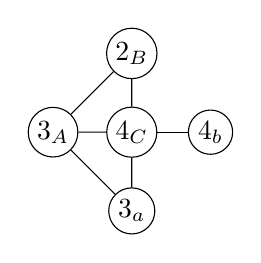
\begin{tikzpicture}[scale=1,every node/.style={draw,circle, inner sep=.05 cm}]
% \foreach \i in {0,1}{
% 	\node (\i1) at (\i-1,\i){$A_{\i}$};
% 	% \node (\i0) at (\i,-1){$h_{\i}$};
% 	}
\node (01) at (-1,0){$3_A$};
\node (11) at (0,1){$2_B$};
\node (02) at (0,0){$4_C$};
\node (0-1) at (0,-1){$3_a$};
\node (03) at (1,0){$4_b$};
\draw (02)--(01)--(11)--(02)--(0-1)--(01);
\draw (02)--(03);
% \draw (01)--(11)--(00)--(01);
\end{tikzpicture}


\[
  \mathbf{\alpha} = 
    \bordermatrix{ & \bar{f_1} & \bar{f_2} & \bar{f_3} \cr
      k_1 & 0 & 0 & 1 \cr
      k_2 & 1 & 0 & 0 \cr
      k_3 & 0 & 0 & 1 \cr
      k_4 & 0 & 1 & 0 } \qquad
\]
\end{document}